%%%%%%%%%%%%%%%%%%%%%%%%%%%%%%%%%%%%%%%%%%%%%%
\section{Beamline}
\label{sec:h4beamline}

%The H4 beamline will be extended to the NP04 cryostat in the newly constructed extension of EHN1. To produce particles in the momentum range of interest, the 80-GeV/c pion beam from the T2 primary target is sent onto a secondary target to generate a tertiary beam. Particles in the tertiary beam are momentum- and charge-selected and transported down the H4 beamline extension into the protoDUNE-SP detector. In principle, the H4 beamline can operate in parallel with the H2 beamline. % minimize interference between the two ProtoDUNE experiments.
%\fixme{H2 and H4 haven't been introduced; unless done in a different section... to check... Anne}
%\fixme{I am moving this to the beginning of the chapter; it can serve as an introduction to it.}
The design of the H4 beamline extension mirrors that of the H2. In this section, we describe the beamline design and the expected beam properties.

%%%%%%%%%%%%%%%%%%%%%%%%
\subsection{H4 beamline layout and optics}

The placement of the quadrupole and dipole magnets in the H4 beamline extension is illustrated in Figure~\ref{fig:H4layout}. The distance from the secondary target to the front of the NP04 cryostat is about 37 m. For the hadron beam, either a tungsten or a copper target will be used. For the electron beam, a Pb target of a few radiation lengths will be used. The first two dipole magnets (shown in red) after the secondary target are rotated by about 56$^\circ$ to steer the beam downward towards the cryostat. The third dipole magnet (shown in green) is used for steering the beam horizontally into one of the three beam positions.
%\fixme{The prev diagram shows the beam windows at the top of the cryostat; this looks like it points lower. Can the beam windows be shown on this image? }

\begin{cdrfigure}[H4 beamline layout]{H4layout}{Layout of the quadrupole and dipole magnets in the H4 beamline extension. The secondary target (not shown) is upstream of the first quadrupole magnet on the left side of the Figure. Vacuum beam pipe and beam instrumentations are also not shown. (Courtesy of V. Clerc, CERN).}
  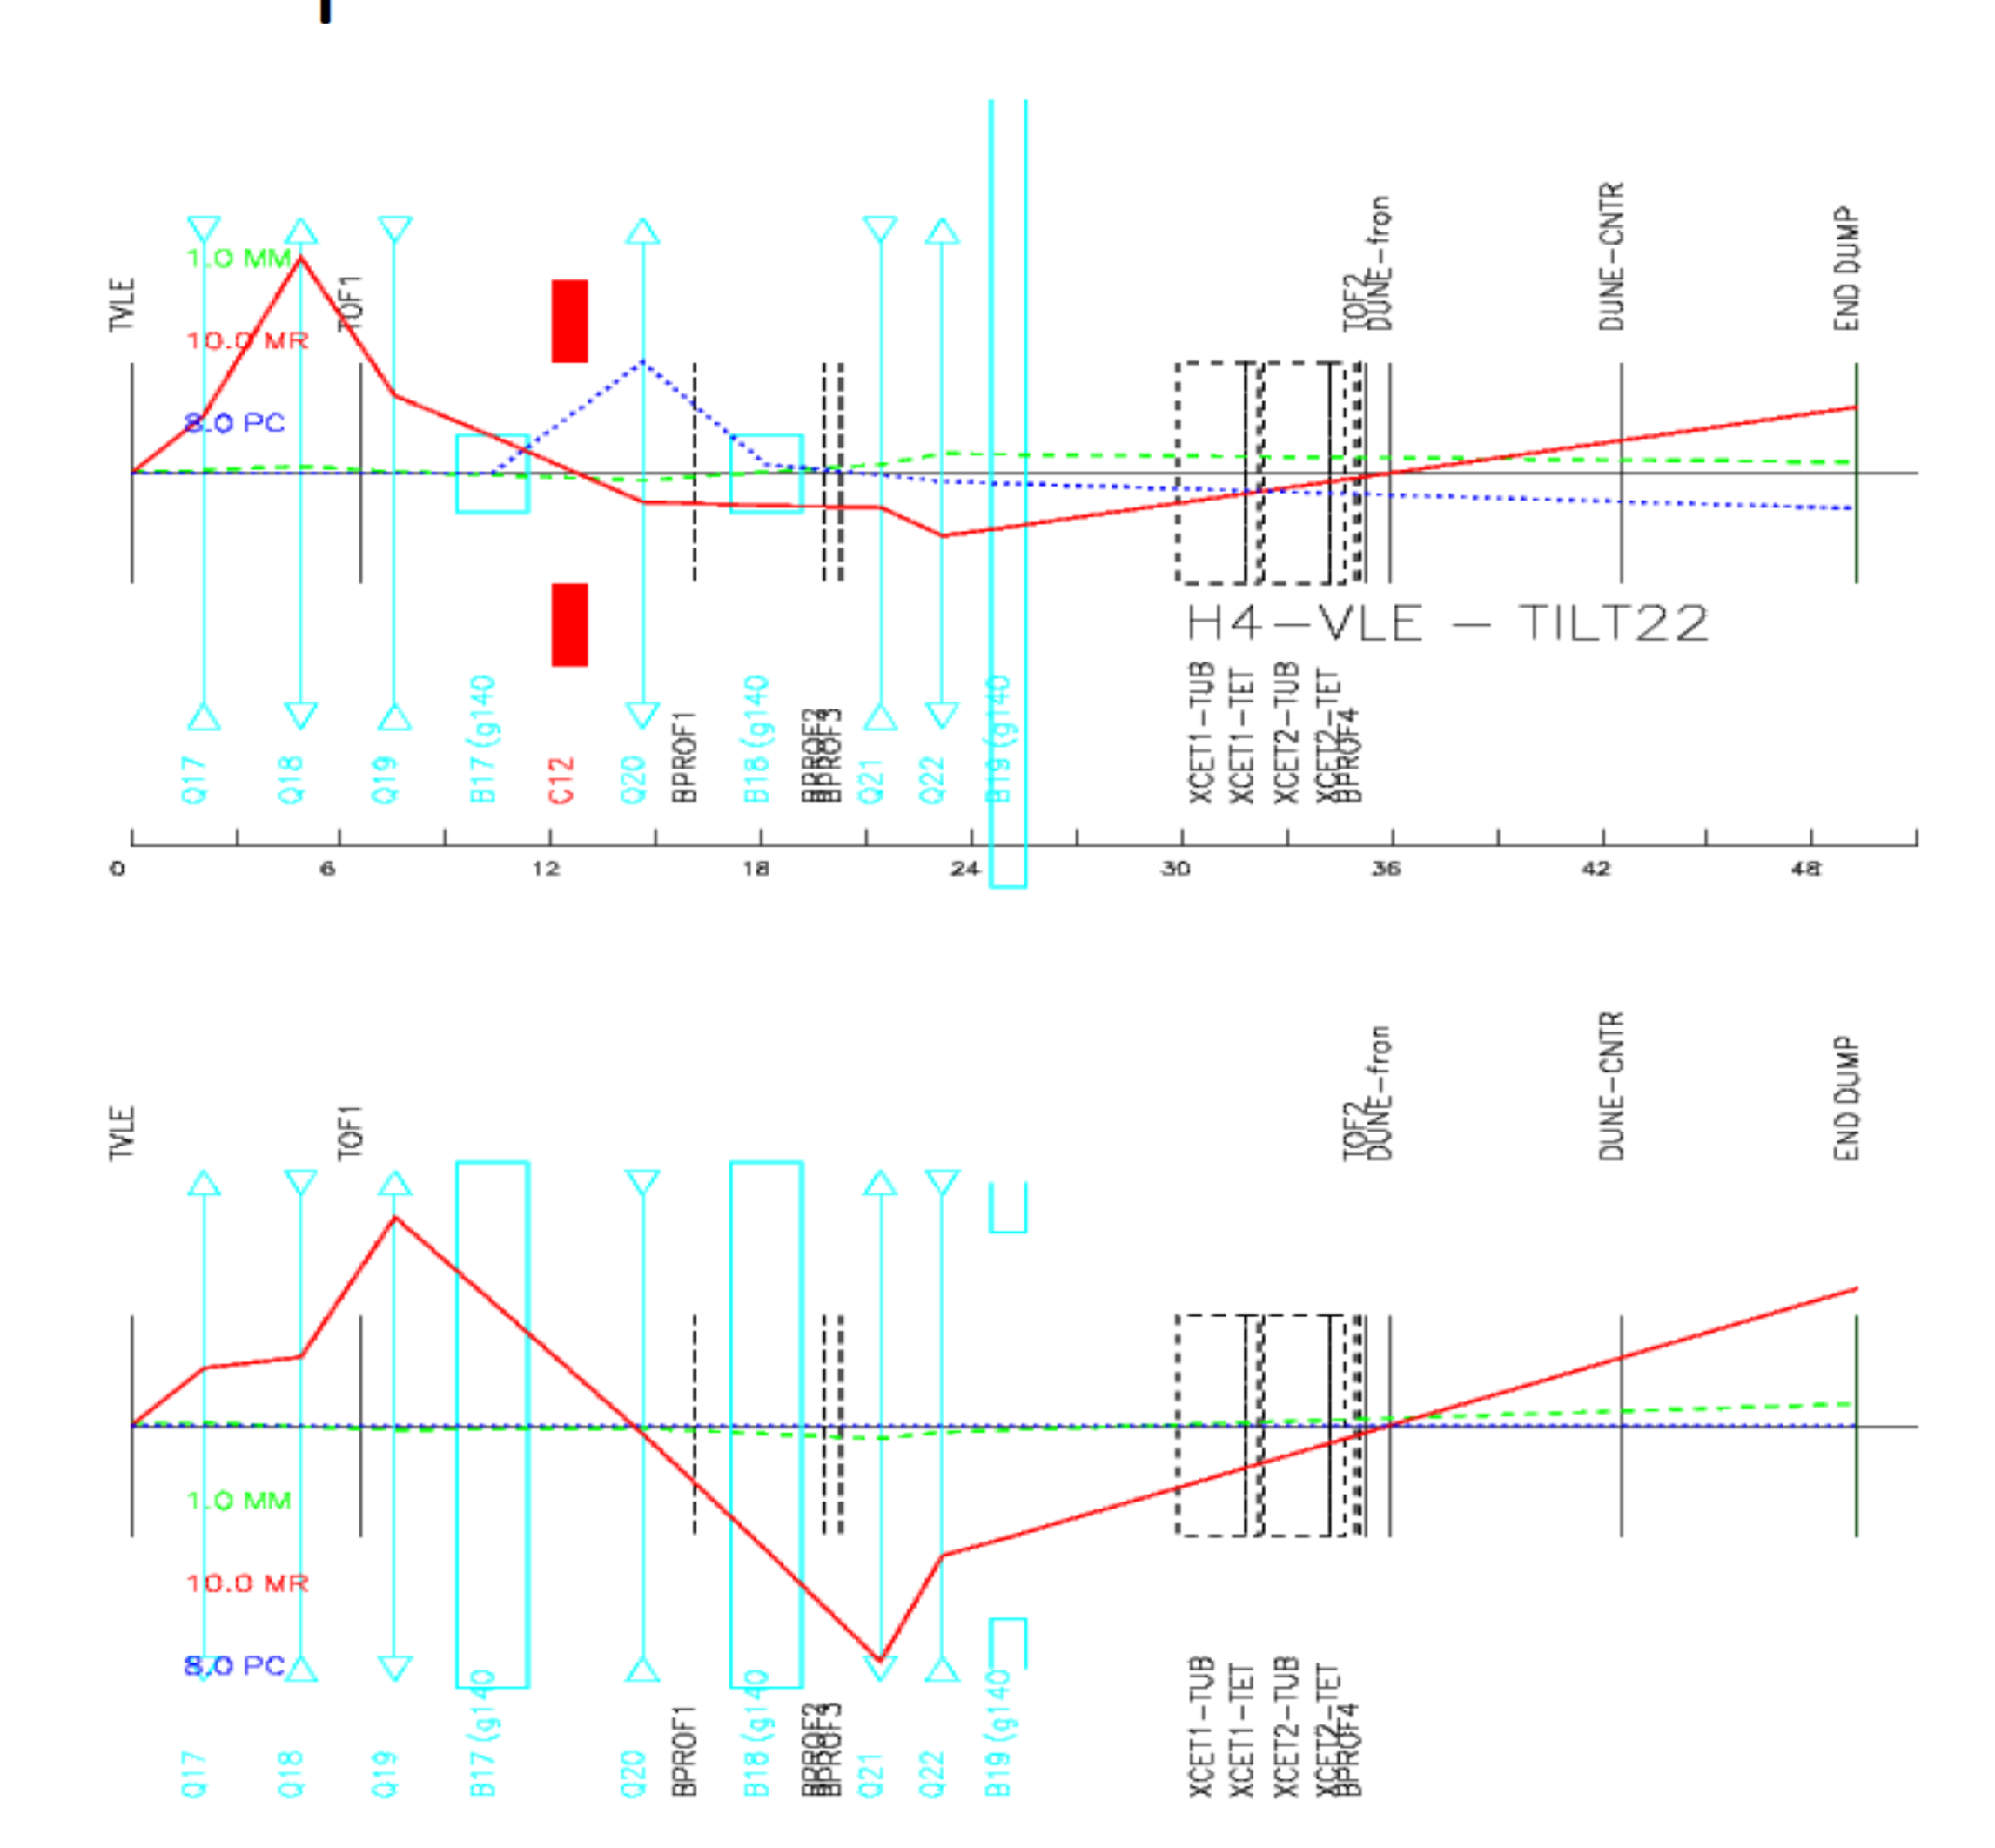
\includegraphics[width=0.75\textwidth]{beamline_H4layout}
\end{cdrfigure}

The beamline optics from the target to the cryostat for the horizontal and vertical planes are shown in Figure~\ref{fig:beamoptics}. The Figures show the position of the quadrupole magnets (Q17-Q22), dipole magnet (B17 - B19), collimator (C12), Time-of-Flight detectors (TOF1-2), beam profile monitors (BPROF1-4), and the Threshold Cherenkov counters (XCET1-2)  relative to the secondary target.  For the nominal configuration, the beam is focused at the front of the cryostat to ensure maximum acceptance of beam particles through the beam window penetration and the beam plug inside the cryostat.

The beamline is in vacuum, with a beam pipe extending from the secondary target down to the beam window in the cryostat upstream face. 

\begin{cdrfigure}[H4 beam optics]{beamoptics}{H4 beamline extension optics for the horizontal (top) and vertical (bottom) planes. The secondary target is located on the left side of the plots and the front of the ProtoDUNE-SP cryostat is located at the beam focus point, at about 37 m from the secondary target. Q17-Q22 are the quadrupole magnets. B17-B19 are the dipole bending magnets. TOF1-2 are the Time-of-Flight detectors, BPROF1-4 are the beam profile monitors, and XCET1-2 are the threshold Cherenkov counters. }
 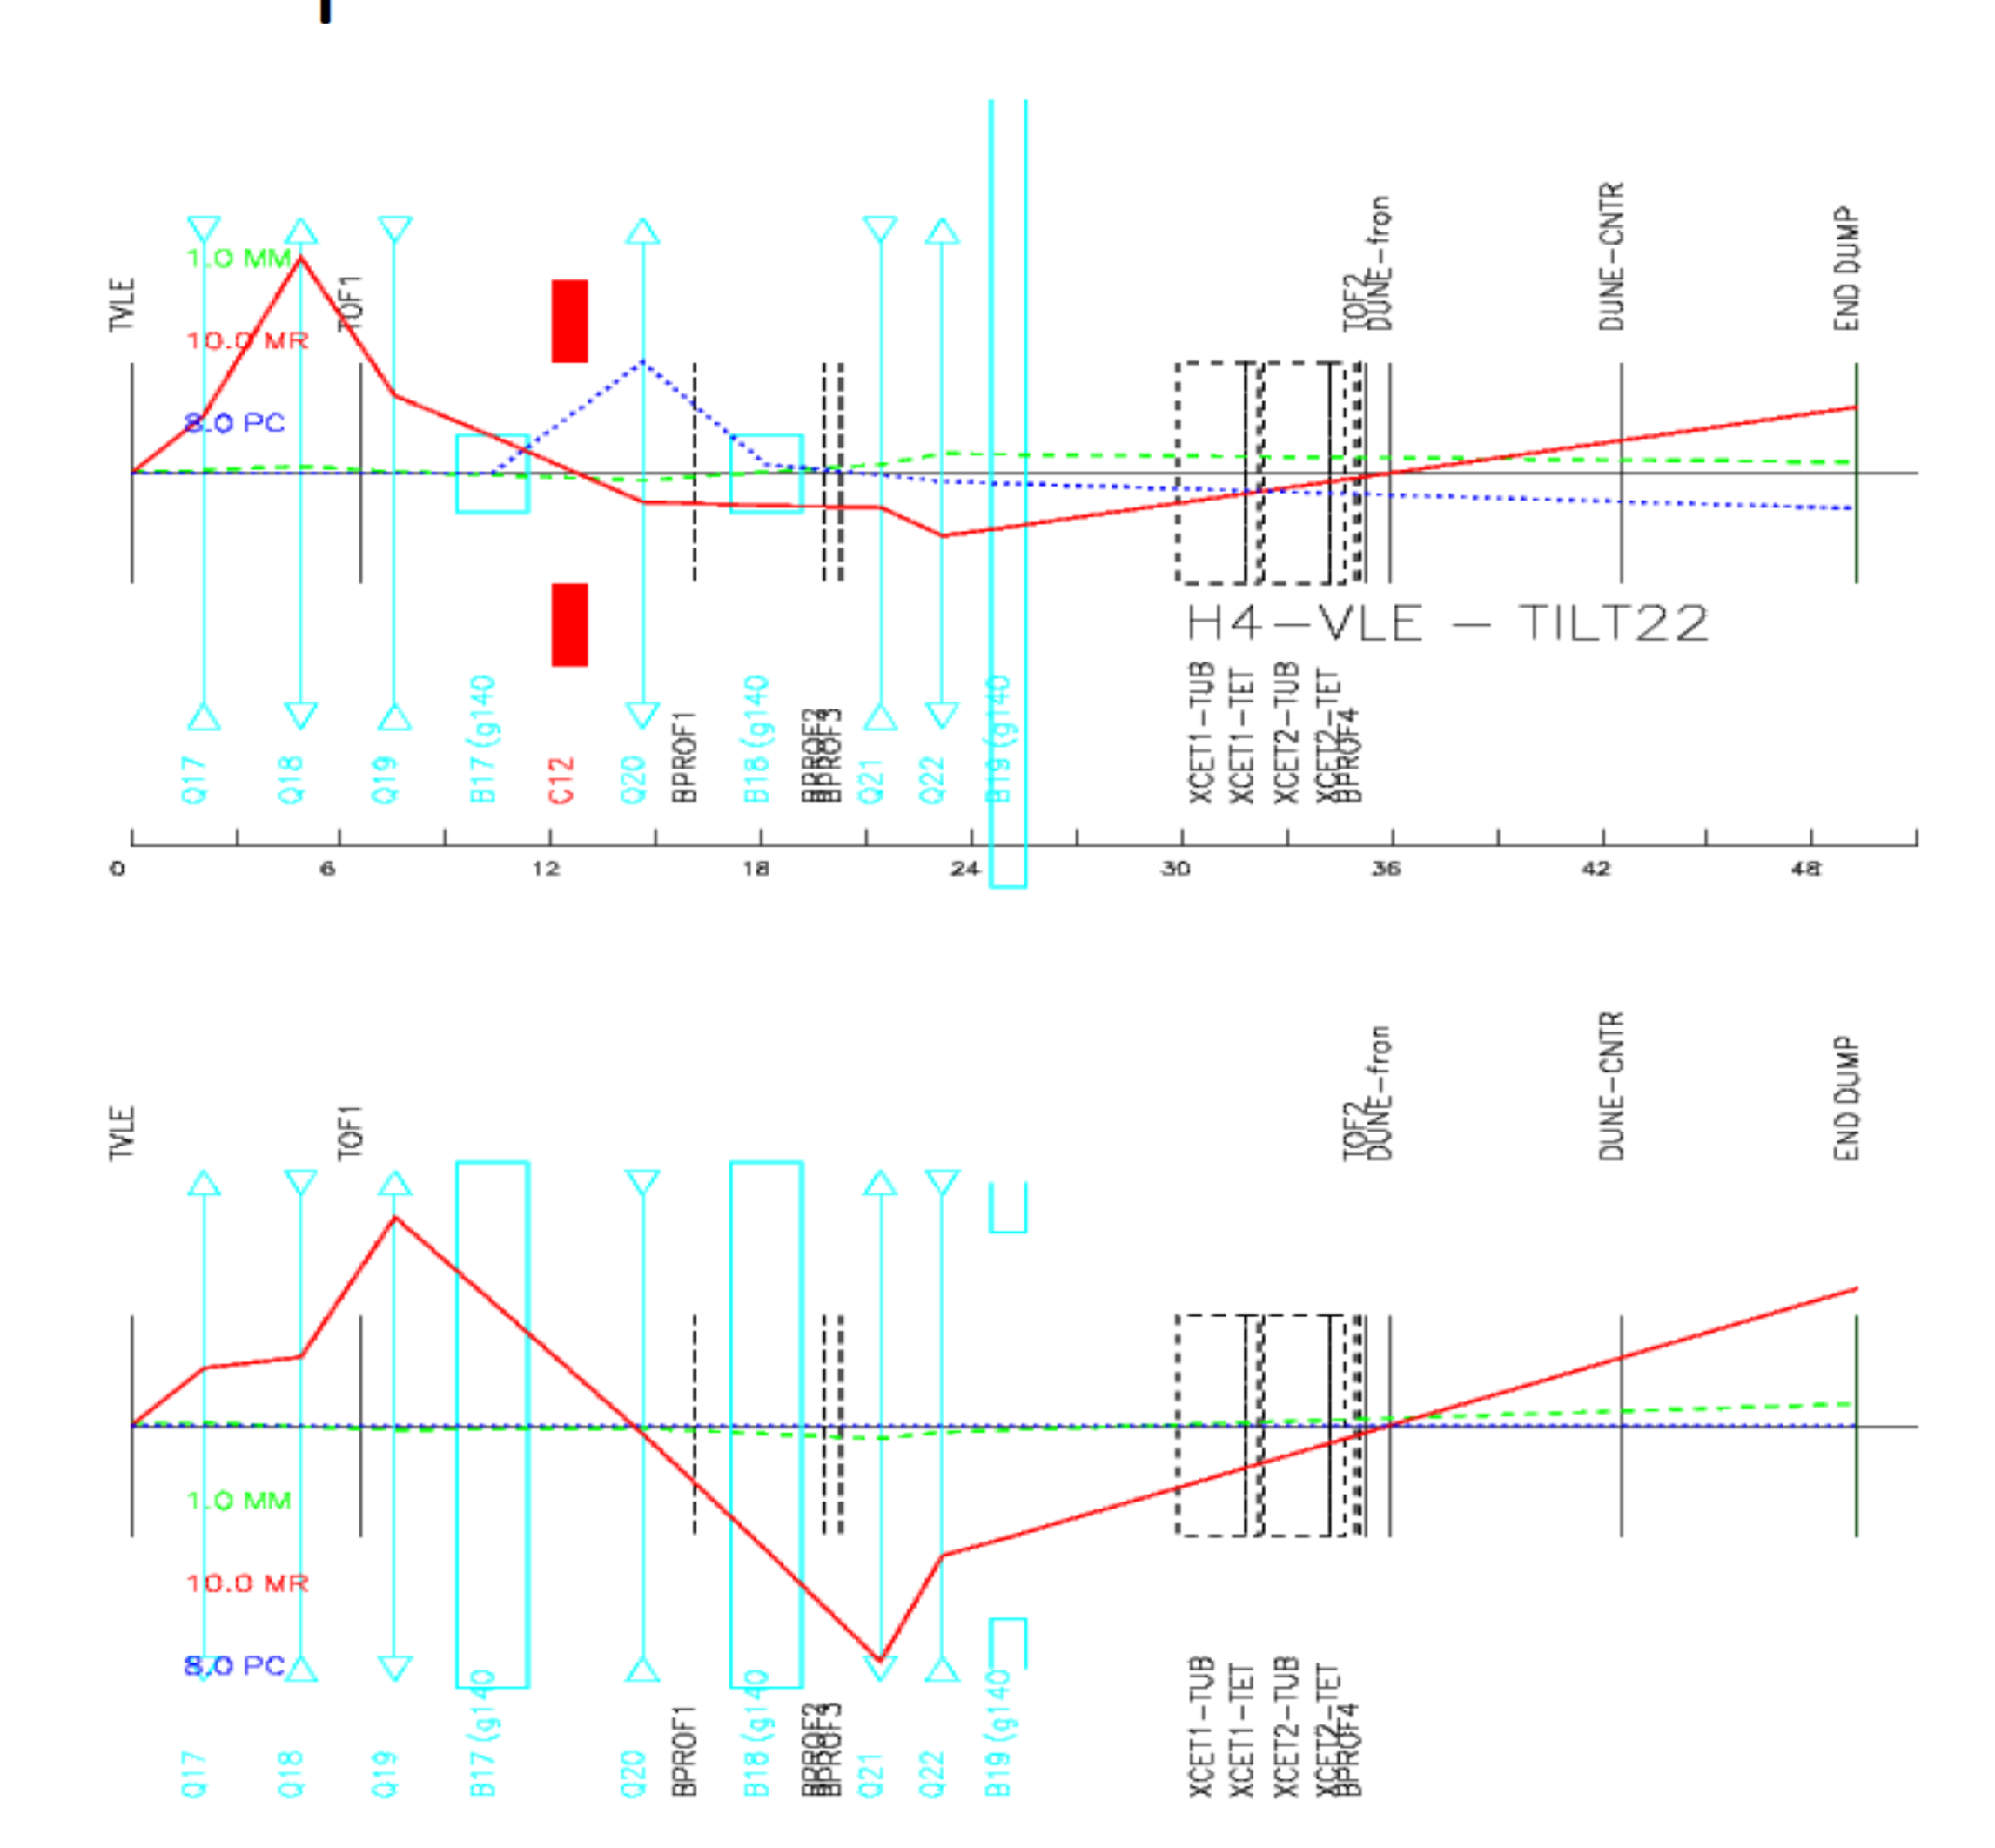
\includegraphics[width=0.99\textwidth]{beamline_H4Optics.pdf}
\end{cdrfigure}
%\fixme{Need to update the beam optic diagram with the version that includes TOF}

%%%%%%%%%%%%%%%%%%%%%%%%
\subsection{Beam properties}
%\fixme{Need simulation results from Nikos -- H4 beam files are available }
A full GEANT4 simulation of the H4 beamline including its extension to the ProtoDUNE-SP detector %cryostat 
has been performed.%~\cite{H4beamfiles}. 
%%%Preliminary results based on the H4 beamline simulation are presented. 
 The beamline model starts with the H4 secondary beamline 
%\fixme{does it also include the primary beam line ?}
%to derive the 
and derives the particle properties in the tertiary beamline.  Target, magnets, collimators and a preliminary assumption
about beam instrumentation are included. The secondary target has been
modeled as a Tungsten cylinder (R=30~mm, L=300~mm) for beam momenta $\leq$~3~GeV/c and as a Copper cylinder of the same dimensions  for beam momenta  $>$~3~GeV/c. Optimization of the target dimensions and material is ongoing.

Table \ref{tab:beampartcomp} describes the particle composition of the
hadron beam at the entrance of the cryostat. Two features are evident. First, the beam is dominated by positrons at low energies,
and secondly, the kaon content, and to a lesser extent the pion content, are depleted at lower energies due to decays of these species 
along the beam path. 

\begin{cdrtable}[Beam composition]{cccccc}{beampartcomp}{Beam composition (in percentage)  at the cryostat entrance for particles contained in the beam pipe (R= 10~cm).}
Momentum (GeV/c) & e$^{+-}$ & $K^{+-}$ & $\mu^{+-}$ & $p^{+-}$& $\pi^{+-}$ \\ \toprowrule
-7  &27.4 &3.4 &1.0 &1.3  &66.9 \\ \colhline
-6  &33.5 &2.9 &1.2 &1.3  &61.2 \\ \colhline
-5  &43.2 &1.9 &1.3 &1.1  &52.5 \\ \colhline
-4  &54.6 &1.1 &1.4 &0.6  &42.3 \\ \colhline
-3  &28.4 &1.1 &2.3 &1.4  &66.8 \\ \colhline
-2  &48.9 &0.3 &1.8 &0.4  &48.6 \\ \colhline
-1  &81.7 &0.2 &1.1 &0.2  &16.9 \\ \colhline
-0.4&98.3 &0.0 &0.4 &0.0  &1.3 \\ \colhline
0.4 &99.1 &0.0 &0.0 &0.5  &0.5 \\ \colhline
1   &69.3 &0.0 &0.3 &15.3 &13.9 \\ \colhline
2   &34.9 &0.6 &1.7 &22.9 &39.0 \\ \colhline
3   &19.9 &2.8 &0.6 &18.9 &56.6 \\ \colhline
4   &47.1 &1.6 &1.1 &8.8  &41.3 \\ \colhline
5   &37.0 &2.8 &0.9 &9.4  &49.5 \\ \colhline
6   &28.1 &4.0 &0.9 &10.4 &56.2 \\ \colhline
7   &20.6 &5.1 &1.0 &10.7 &62.6 \\
\end{cdrtable}
%
Particle rates, assuming a spill intensity of $10^6$
particles on the secondary target and a SPS spill length of 4.8
seconds, are reported in Table~\ref{tab:beampartrates}. The H4 simulation results are documented in CERN-ACC-NOTE-2016-0052. 
%\fixme{What does "achievable" mean here ? e.g. is some special tweaking required to achieve these rates or is this some average coming out of the calculation.}
\begin{cdrtable}[Particle rate]{ccccccc}{beampartrates}{Particle rates (Hz).}
Momentum (GeV/c) & e$^{+-}$ & $K^{+-}$ & $\mu^{+-}$ & $p^{+-}$& $\pi^{+-}$& total\\ \toprowrule
-7  & 57 & 7  & 2  & 3  & 138& 207 \\ \colhline
-6  & 62 & 5  & 2  & 2  & 113& 185 \\ \colhline
-5  & 72 & 3  & 2  & 2  & 87 & 166 \\ \colhline
-4  & 93 & 2  & 2  & 1  & 72 & 170 \\ \colhline
-3  & 11 & 0.5& 1  & 0.5& 26 & 39 \\ \colhline
-2  & 13 & 0  & 0.5& 0.1& 16 & 27 \\ \colhline
-1  & 18 & 0  & 0.2& 0  & 4  & 22 \\ \colhline
-0.4&  8 & 0  & 0  & 0  & 0.1& 8 \\ \colhline
0.4 & 7  & 0  & 0  & 0  & 0  & 7 \\ \colhline
1   & 18 & 0  & 0  & 4  & 4  & 27 \\ \colhline
2   & 13 & 0.2& 0.5& 9  & 15 & 38 \\ \colhline
3   & 11 & 1  & 1  & 11 & 31 & 56 \\ \colhline
4   & 92 & 3  & 2  & 17 & 81 & 196\\ \colhline
5   & 74 & 6  & 3  & 19 & 99 & 200\\ \colhline
6   & 63 & 9  & 3  & 24 & 127& 226\\ \colhline
7   & 52 & 13 & 2  & 27 & 157& 252\\
\end{cdrtable}
%\fixme{Caption of table 7.3 says "trigger rates" whereas text says "particle rates". Unify language, I think it should be particle rates.}
%\fixme{what are the units for the rates in table 7.3 ?}

At momenta larger than about 4 GeV/c, the particle rates are at the limit or beyond the DAQ capability.
 At lower energies, the proton and pion rates are much lower, reduced by a
factor of 10 at 1 or 2 GeV/c, and are overwhelmed by the positron rate.

The momentum spread of the beam is of the order of 5--7\%. At higher energies, where
the particle rate is higher, the momentum spread  can be narrowed by
closing the collimators, at the expense of the beam intensity.  For example, Figure \ref{fig:momcoll} shows
that at $p=4$~GeV/c the momentum spread can be  reduced to $\Delta p/p= 3.6\%$ with a factor of 4 reduction in particle rate.  
\begin{cdrfigure}[Beam momentum uncertainty]{momcoll}{Beam momentum spread with different collimator openings at 4 GeV/c.}
  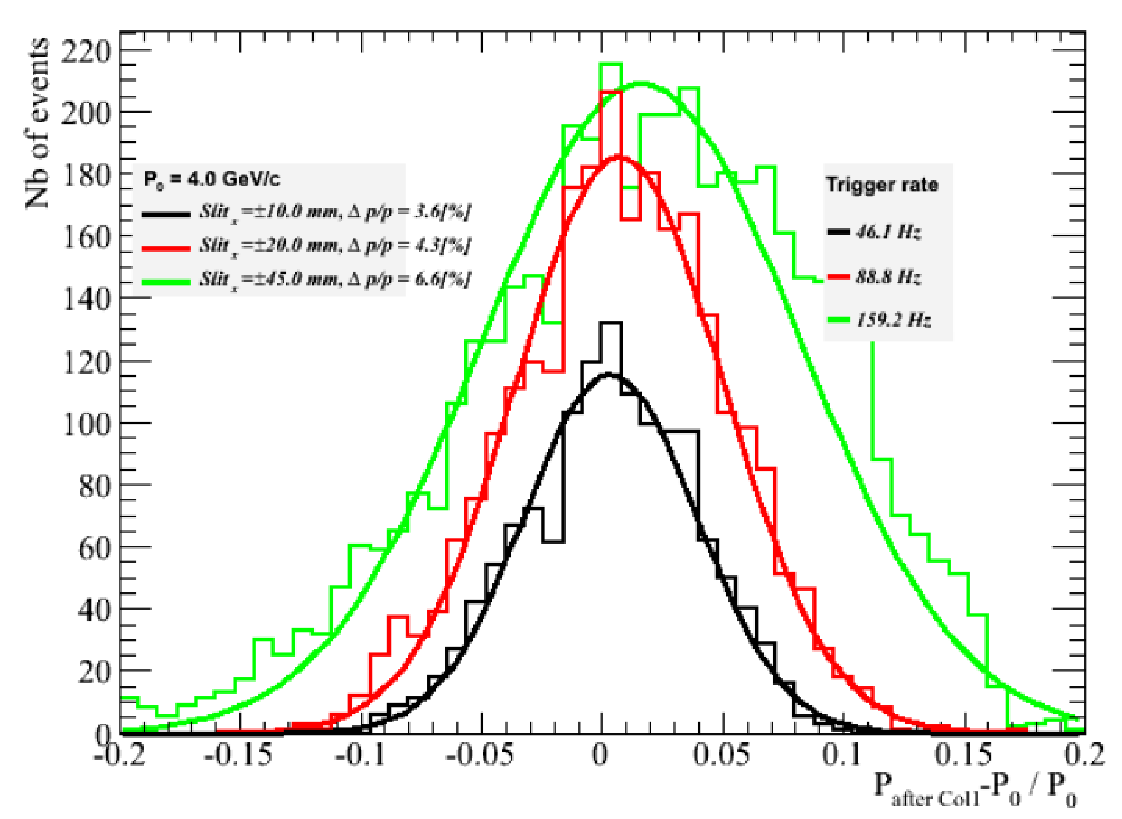
\includegraphics[width=0.75\textwidth]{Slits.pdf}
\end{cdrfigure}
%\fixme{increase size of legend in figure; change trigger rate to particle rate in figure}
%\fixme{How are the values of 3.6, 4.3 and 6.6\% obtained ? Not obvious from figure.}
%\fixme{ Figure from Nikos, need him to redo it}


%%%%%%%%%%%%%%%%%%%%%%%%
\subsection{Muon halo}
The secondary beam is mainly composed of 80-GeV pions. In the long path ($\approx$ 600~m) between the primary and the secondary target,
 an intense high-energy muon halo is produced by pion decay. Muons propagate approximately in the direction of the first section of the H4 beamline,  that is slightly upward  and sidewards of the H4 beamline extension which points at the ProtoDUNE-SP detector.  
 Therefore the most intense part of the muon halo passes about one meter above the left corner of ProtoDUNE-SP cryostat. 
Figure~\ref{fig:muonhalo_HE} shows the spatial distribution of the muon halo at the face of the cryostat. Only muons with momentum larger than 4~GeV/c have been considered. Despite the low statistics of the simulations, the up-down and left-right asymmetry is clearly visible. 
The origin of the coordinate system is chosen to coincide with the center of the cryostat face. The color scale shows the muon intensity in  $\mu/m^2/$spill for $10^6$ particles/spill from the primary target. The muon intensity on the cryostat face, indicated by the black rectangle in Figure~\ref{fig:muonhalo_HE}, ranges up to $\sim$400~$\mu$/m$^2$/spill. However, the rate of halo muons impinging on the front side of the TPC active volume (red rectangle) is expected to be significantly lower, in particular, as low as a few $\mu$/m$^2$/spill on the Saleve side of the TPC 
where the H4 beamline points. The rate of beam events with out-of-time halo muon tracks captured in the 2.5 ms time frame of the recorded event is expected to be limited.

Figure~\ref{fig:muonhalo_HE}  is very preliminary though, not only because of low statistics, but also because shielding around the low-energy beamline is not included in the simulation, and the muons produced in neighboring beamlines in EHN1, including the H2 beamline that feeds ProtoDUNE-DP, are not considered here. Based on these results, the estimated contribution to the total data volume from beam halo is negligible.
\begin{cdrfigure}[Muon halo intensity at the cryostat face]{muonhalo_HE}{Muon halo intensity at the cryostat face for muons originating from the H4 beamline and with $P_\mu  \ge 4$~Gev/c. The origin of the $x-y$ coordinate system is centered on the cryostat and dimensions are in mm. Color scale is in units of $\mu/m^2/$spill. The black and red rectangles represent the cryostat face and front face of the active detector volume.}
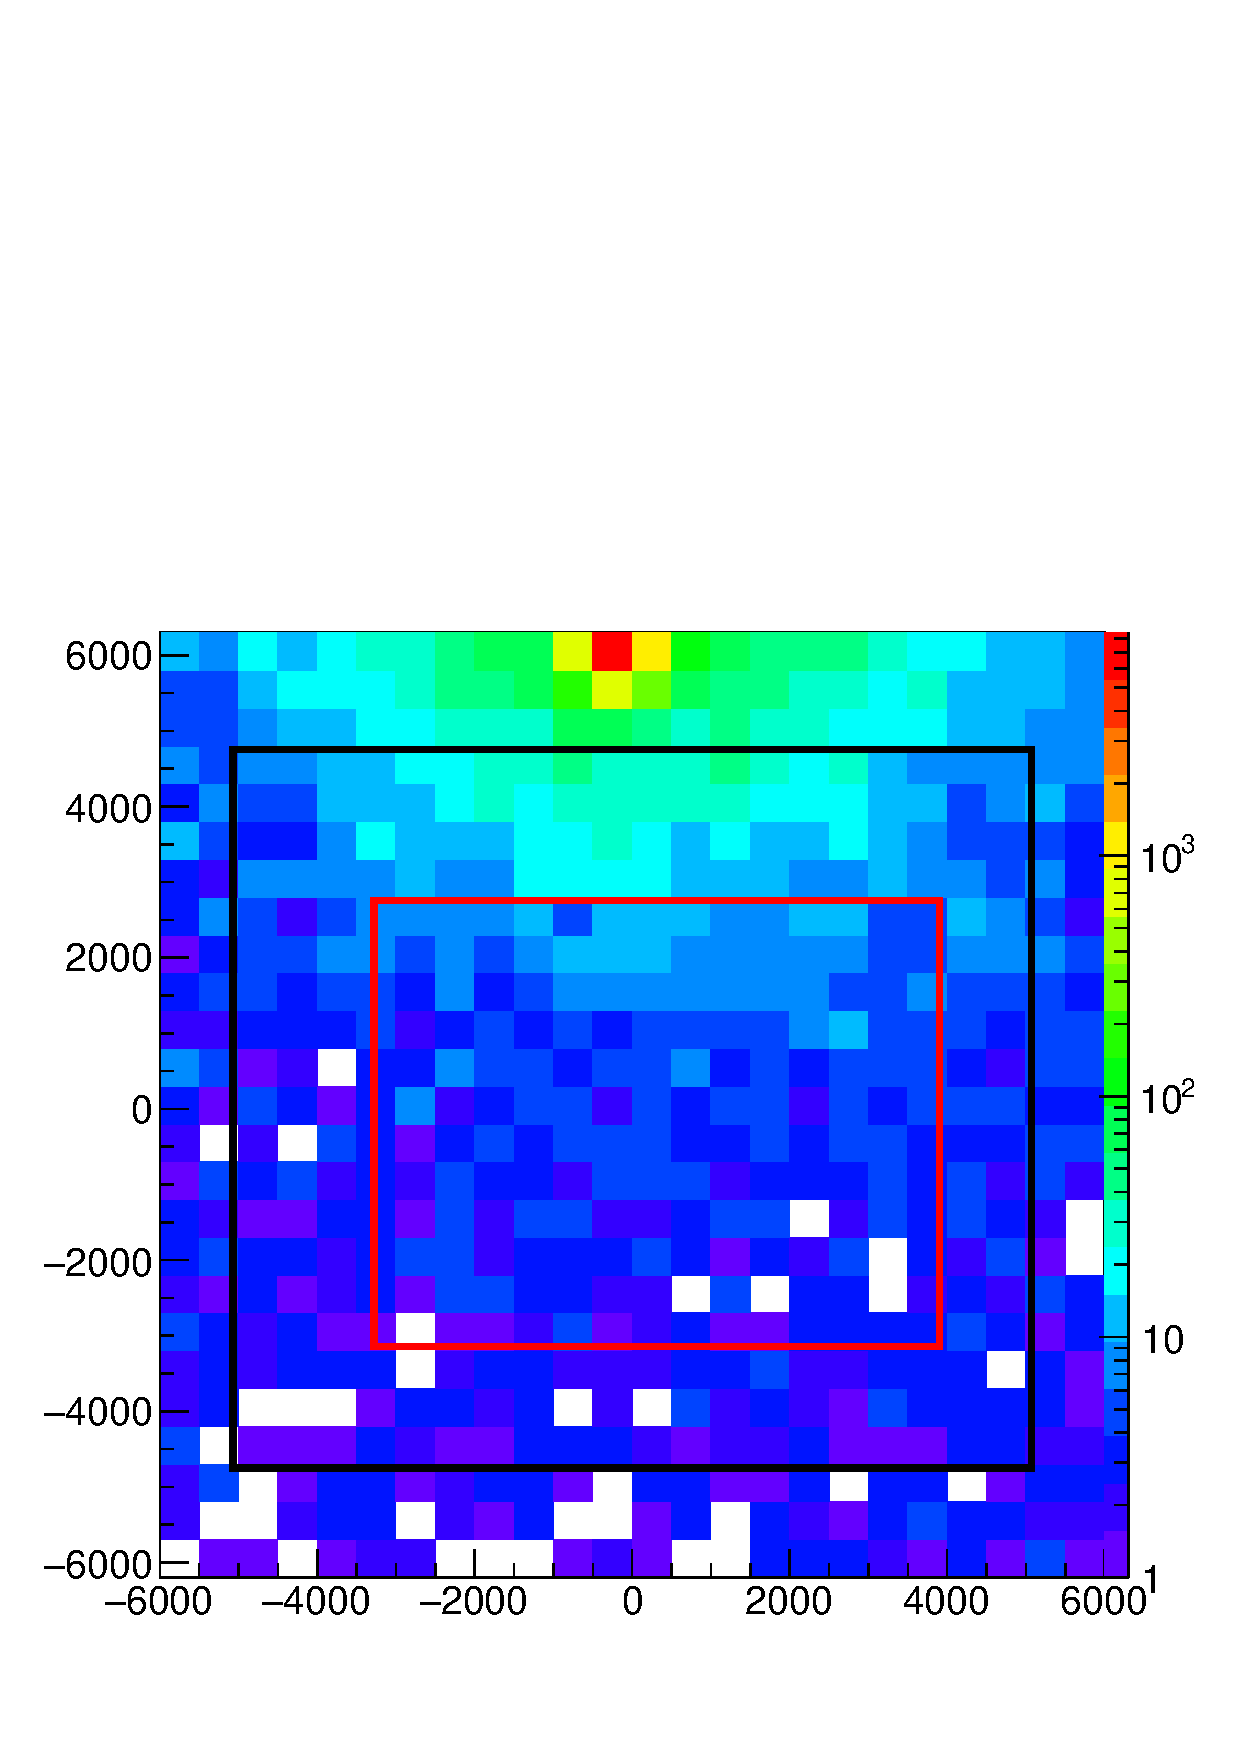
\includegraphics[width=0.50\textwidth]{muon_map_HE_square.pdf}
\end{cdrfigure}
